%! TeX program = lualatex
\documentclass[a4paper,11pt]{article} 
% packages
\usepackage{fontspec}
\setmainfont{EB Garamond}
% for tironian et fallback
% % \directlua{luaotfload.add_fallback
% % ("emojifallback",
% %      {"Noto Serif:mode=harf"}
% % )}
% % \setmainfont{EB Garamond}[RawFeature={fallback=emojifallback}]

\setmonofont[Scale=MatchLowercase]{Deja Vu Sans Mono}
\usepackage[a4paper,left=2cm,right=2cm,top=\dimexpr15mm+1.5\baselineskip,bottom=2cm]{geometry}
\setlength{\parindent}{0pt}

\usepackage{fancyhdr}       % Headers and footers 
\fancyhead[R]{\normalfont \leftmark}
\fancyhead[L]{}
\pagestyle{fancy}

\usepackage{amsmath}
\usepackage{microtype}      % Slightly tweak font spacing for aesthetics
\usepackage[english]{babel} % Language hyphenation and typographical rules
\usepackage[final, colorlinks = false, urlcolor = cyan]{hyperref} 
\usepackage{changepage}     % adjust margins on the fly

\usepackage{minted}
\usemintedstyle{algol_nu}
\usepackage{xcolor}

\usepackage{pgfplots}
\pgfplotsset{width=\textwidth,compat=1.9}

\usepackage{caption}
\newenvironment{code}{\captionsetup{type=listing}}{}
\captionsetup[listing]{skip=0pt}
\setlength{\abovecaptionskip}{5pt}
\setlength{\belowcaptionskip}{5pt}

\usepackage[yyyymmdd]{datetime}
\renewcommand{\dateseparator}{--}

\renewcommand{\labelenumii}{\arabic{enumi}.\arabic{enumii}}

\usepackage{titlesec}

\author{Andrew Hayes, Conor McNamara, Maxwell Maia}

\begin{document}
\begin{titlepage}
    \begin{center}
        \hrule
        \vspace*{0.6cm}
        \huge \textbf{CT3532 Database Systems II}
        \vspace*{0.6cm}
        \hrule
        \LARGE
        \vspace{0.5cm}
            Assignment 2: Indexing
        \vspace{0.5cm}
        \hrule
            
        \vfill
        %
\includegraphics[width=\textwidth]{images/uniog.jpg}
        \vfill

        \Large
       \vspace{0.5cm}
       \hrule
       \vspace{0.5cm}

        \raggedright
        \begin{minipage}{0.329\textwidth}
        \centering
        \textbf{Andrew Hayes}
        
        \normalsize
        Student ID: 21321503
        \end{minipage}
        \begin{minipage}{0.329\textwidth}
        \centering
        \textbf{Conor McNamara}
        
        \normalsize
        Student ID: 21378116
        \end{minipage}
        \begin{minipage}{0.329\textwidth}
        \centering
        \textbf{Maxwell Maia}
        
        \normalsize
        Student ID: 21236277
        \end{minipage}

        \centering
        %\today

        \vspace{0.5cm}
        \hrule
    \end{center}
\end{titlepage}

\pagenumbering{roman}
\newpage
\tableofcontents
\newpage
\setcounter{page}{1}
\pagenumbering{arabic}

\newpage
\section{Indexing Approach \& Algorithm}
\subsection{Indexing Approach}\label{sec:indexingapproach}
\label{indexing}
To construct a heatmap which describes the location of a player over the course of a game, we need to be able to retrieve the number of times a player was in a given location over the course of a game.
We are given a data file for any given game that is already sorted in temporal order containing the timestamp, a triple containing a player's ID \& their $(x,y)$ co-ordinates, and a triple containing the $(x,y,z)$ co-ordinates of the football.
\\\\
We decided to make use of an indexing approach that was optimised specifically for facilitating queries about the amount of time a given player spent in a certain location.
We took advantage of the fact that the data is already sorted in temporal order, which saves us from having to sort the data at all. 
At a high level, our indexing approach involved creating one table for each player-location pair, resulting in many tables, each containing one entry for each recorded instance of that particular player being in that particular location.
The location of the tables on the disk is determined by a hash function, with a hash on the player-location pair, allowing fast lookup. 
\\\\
Our proposed indexing approach is as follows:
\begin{enumerate}
    \item   Define the grid cells that we will be examining for the creation of the heatmap. 
            The number \& size of these cells doesn't really matter from an algorithmic perspective, but the smaller / more numerous they are, the more tables we are going to need and the fewer grids we have, the less precise the heatmap data.
            We can either define a custom number of grids, or we could take the grids that have already been defined for the gathering of the data -- each $(x,y)$ being a grid. 
            The trade-off here is either having a less precise heatmap but with fewer tables, or a more precise heatmap with many more tables.
            If we take, for example, the dimensions of Croke Park (rounded for convenience) $145 \times 90$ metres, we can split the pitch into thirty $29 \times 15$ metre grid cells, as shown below.
            This gives what we felt was a reasonable balance between precision \& having many tables, but  these dimensions could be easily changed as needed for a practical implementation. 
            If we wanted ultimate precision, we could take each co-ordinate recorded in the data file to be a ``grid''.
            \begin{figure}[H]
                \centering
                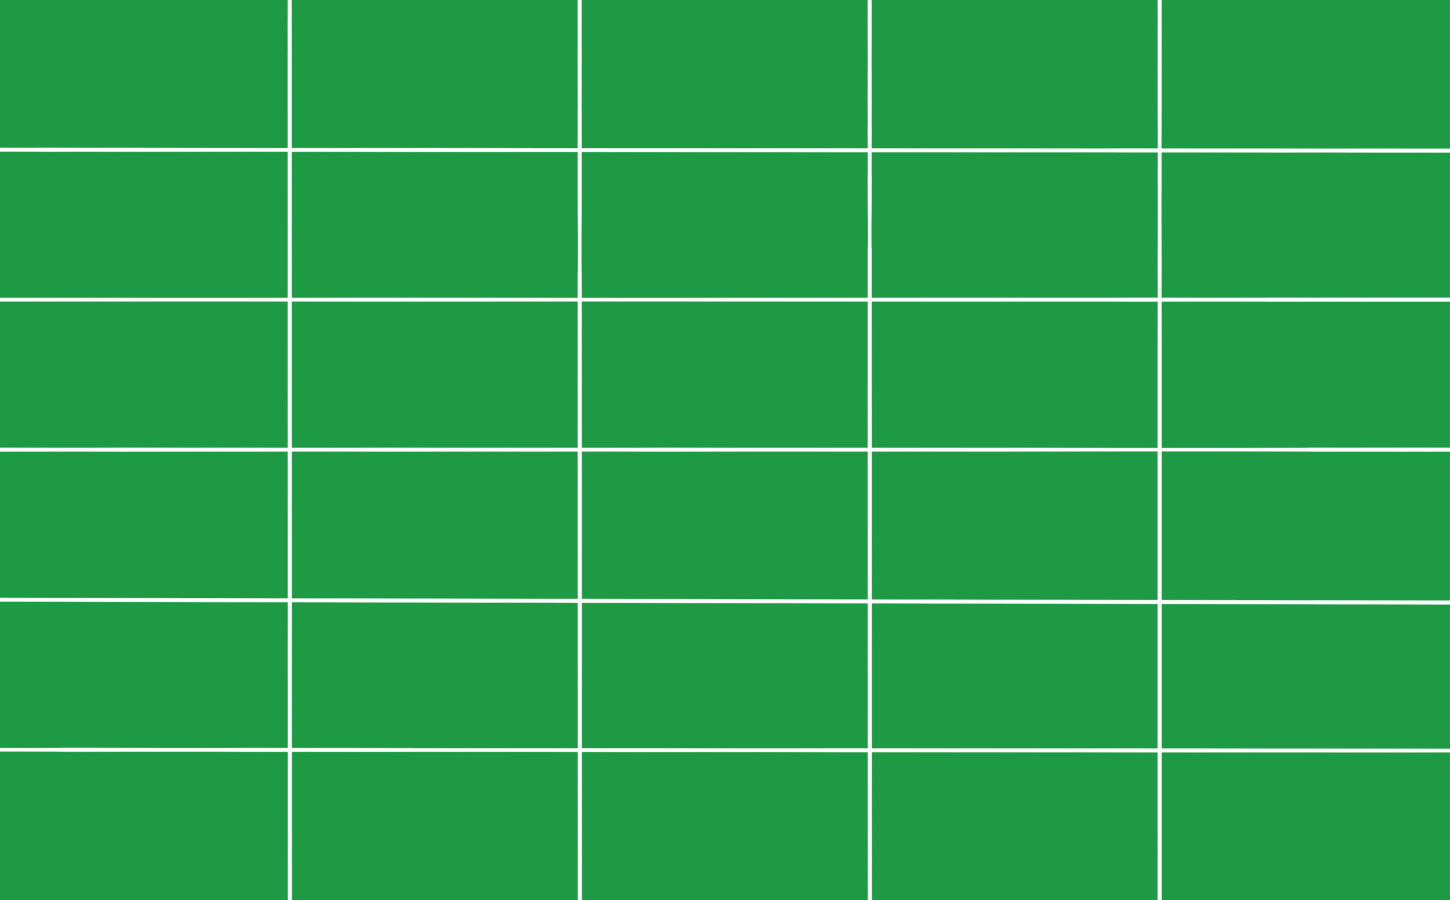
\includegraphics[width=0.7\textwidth]{./pitch.png}
                \caption{A $145 \times 90$ Metre Pitch Split into Thirty $29 \times 15$ Metre Grid Cells}
            \end{figure}
            
    \item   Define a function which returns the grid cell given an $(x,y)$ pair. 
    We identify each grid with a name in the format \verb|x.y| where \verb|x| identifies the number of the column in which the grid is found (counted from left to right in the above figure) and \verb|y| is the number of the row in which the grid is found (counted from bottom to top in the above figure), e.g. the bottom left-hand grid would be referred to as \verb|0.0| and the top right-hand grid would be referred to as \verb|5.6|.
    The following is a possible Python implementation of such a function, for our chosen pitch \& grid dimensions, assuming that the $x$-axis of the pitch is the long side and that $(x,y)$ co-ordinates of a player are just the number of metres that the player is from the bottom left-hand corner on the $x$ \& $y$ axes. 
\begin{code}
\begin{minted}[texcl, mathescape, linenos, breaklines, frame=single]{Python}
# input: a pair of (x,y) co-ordinates 
# output: a string that identifies the grid
def determine_grid(x, y):
    grid_width = 29      # width of each grid in metres
    grid_height = 15     # height of each grid in metres

    # determining the location of the grid using floor division
    grid_x = x // grid_width 
    grid_y = y // grid_height 
    
    # return the grid identifier in the format `x.y`
    return str(grid_x) + "." + str(grid_y)
\end{minted}
\caption{\texttt{determine\_grid()}}
\end{code}

    \item  Define a hash function $h(\texttt{player\_id}, \texttt{grid}) \rightarrow i$ which hashes the player's ID \& the grid identifier together to generate the index $i$ which is the location of the table pertaining to that player-grid pair on the disk.
            This table will be used to record each instance of the player being in that grid throughout the match. 
            Because this overall approach results in the generation of a great number of tables ($\# \text{players} \times \# \text{grids}$), it is important to have a strong hash function that minimises the chances of a collision occurring. 

    \item   For each tuple in the data file:
            \begin{enumerate}
                \item   Identify the grid which contains the player's co-ordinates using the \mintinline{python}{determine_grid(x,y)} function, supplying the player's $x$ \& $y$ co-ordinates to the function as arguments.
                \item   Hash the player's ID \& the grid identifier together using $h(\texttt{player\_id}, \texttt{grid})$ to generate the index $i$ of the table pertaining to that player-grid pair on the disk. 
                \item   Store the minimum data required from the original tuple in the table at index $i$, creating the table if it does not already exist. 
                        Because we are iterating over data that is already sorted by timestamp, our insertions into the database will also be sorted, saving us from having to sort them ourselves.   
                        We will calculate the amount of time spent in the grid by the number of entries in this table, so we assume that the data is always recorded at a regular interval, say 100ms. 
                        The amount of time spent in the location will then be calculated by multiplying the count of entries in that table by the interval at which data was recorded, e.g. if the interval was 100ms and there were 6000 entries in the table, then we could say that the player spent $6000 \times 100 = 600000$ milliseconds in that location (ten minutes).
                        The obvious downside of this approach is that if data is not always recorded at a regular interval, it will not work. 
                        In that case, we could additionally store the amount of time that elapsed before the next entry for that player was recorded in the data file as a column in the table. 
                        This would of course require extra processing, as we would have to seek out the next instance of the player ID in the data file, get the timestamp of that entry, and then subtract the timestamp of the current entry from the timestamp of the next recorded timestamp for that player to calculate the interval, but it would allow a similar querying approach: to calculate the amount of time a player spent in the location, we could just sum the values in that column.
                        \\\\
                        The minimum data required will vary depending on the type of queries that we intend to execute; theoretically, if the only thing we wanted to know was the amount of time that a player spent in the grid and the data was always recorded at regular intervals, we could get away with not storing any data other than an iterative ID for each row that counts the number of times the player was recorded in that location. 
                        We decided not to opt for this approach, instead opting to store everything from the original tuple except the player's ID (as that is implicit for the table), which allows us to execute the maximum number of different queries that we can, such as querying the distance from the player to the ball when the player is in that location for example.
                        Alternatively, we could also just store a pointer to the original tuple in the data file in the table, thus ensuring there is no duplication of data but we decided against this as it would require each tuple to be parsed for every query executed, rather than just parsing the tuples out into their respective columns once. 
            \end{enumerate}
\end{enumerate}

\subsection{Algorithm}
Our proposed algorithm for calculating the amount of time that a player spent at a given location is largely outlined above, but we will lay it out here in a more concise manner. 
Given the player's ID and either a pair of $(x,y)$ co-ordinates in the desired location, or the grid identifier of the given location: 
\begin{enumerate}
    \item   Identify the grid location, if not given, using the \mintinline{python}{determine_grid(x, y)} function given above.
    \item   Get the index $i$ of the player-grid table using $h(\texttt{player\_id}, \texttt{grid})$.
    \item   Query the length of the table at index $i$.
    \item   Multiply the length of the table $L$ by the interval at which data was recorded $\Delta$ to get the time spent in the grid $t = L \times \Delta$.
            E.g., if $\Delta = 100\text{ms}$ and $L = 6000$, then the amount of time spent in the grid is $t = 6000 \times 100 = 600000\text{ms}$, or ten minutes.
\end{enumerate}

\section{Parallelisation}
One advantage of the chosen approach is that it relies on \& maintains the sorted order of the original data file when entering data into the tables.
Although the tables being in order is not strictly necessary for the primary type of query we are discussing here (querying the amount of time that a player spent at a location over the course of a game), it is highly advantageous to have the tables already in sorted order, as it saves us from having to sort them if we wanted to, for example, query the amount of time a player spent in a location in the second half of the match.
For this reason, we will want to ensure that the temporal order of the data is maintained when parallelising the approach.
\\\\
We could split the data file into $n$ equal chunks, where $n$ is the number of CPUs available, and then have each CPU apply the approach outlined above to process their chunks, but then the data would not be inserted into each table in sorted order; we would then have to sort each table using in some manner (such as a two-pointer approach) to end up with the sorted tables.
Instead, to keep in line with our existing indexing approach, and maintain the sorted order of the data file from the beginning, we opted for the following approach:
\begin{enumerate}
    \item   Iterate over the data file and pull out the set of player IDs contained within it, e.g. for a match of Gaelic Football with no substitutions, we would have $30$ player IDs.
    \item   Assign each CPU available to us a set of player IDs that it will be responsible for, ensuring no overlap. 
            The split of the player IDs among the CPUs should be as equal as possible, assuming equally powerful CPUs.
    \item   For each player ID in its set, each CPU will iterate through the data file in order, searching for the tuples which contain the player ID currently under consideration.    
            Each tuple will be handled with the approach outlined previously (identify grid, get index of player-grid table, insert data).
            This maintains the primary advantage of the original indexing approach: we take advantage of the data already being sorted and avoid having to re-sort it.
\end{enumerate}


% ## Parallelize query ?
% - Split the return table from hash(p_id, grid cell) into chunks and assign to different CPUs using round robin (as just want an equal split of work between CPUs)

\section{\boldmath{$3 \times 3$} Grid Heatmap}\label{sec:heatmap}
The indexing approach outlined in the section \textbf{\hyperref[sec:indexingapproach]{Indexing Approach}} would work for the coaches' queries about the times in which a given player was in a specified rectangle of the $3 \times 3$ grid.
The indexing approach would be completely unchanged, except the grid definitions would be different, with both different grid dimensions and a different number of tables. 
For each tuple in the data file, the grid would be identified from the $(x,y)$ co-ordinates using the \mintinline{python}{determine_grid()} function, the player ID \& the grid identifier would be hashed together to find the location of the relevant table on disk, and the data would be inserted. 
The number of times that a player was in a given grid could be determined by simply hashing the player ID \& the grid identifier together to get the location of the relevant table on disk, and querying the length of that table to find the number of entries. 
\\\\
The following pseudo-code could be used to calculate the values for a heatmap for each player across the entire pitch:
\begin{code}
\begin{minted}[texcl, mathescape, linenos, breaklines, frame=single]{Python}
# function to determine the number of times a given player was in a given grid 
# input: player ID, grid identifier 
# output: count of the number of times that player ID was recorded in that grid
def player_grid_values(player_id, grid_id):
    # get table location on disk
    table_location = hash(player_id, grid_id)

    # query the number of rows in that table using some pseudo-SQL nonsense
    count = select("count(*) from table @ " + table_location)  

    return count

# function to generate a an array of heatmap values for every location on the pitch
# input: an array of locations on the pitch, an array of the player IDs in the game
# output: an array numbers indicating the number of times a player was in each location
def generate_heatmap(locations, players):
    # output array will hold the number of times a player was in each location, in the same order as the locations array
    heatmap_values = [] # assume each index initialises to 0

    # iterate over each location
    for (int i = 0; i < locations.length; i++):
        # iterate over each player for each location
        for (int j = 0; j < players.length; j++):
                player_id = players[j]
                heatmap_values[i] += player_grid_values(player_id, location)  
\end{minted}
\caption{Pseudo-Code to Calculate the Heatmap Values}
\end{code}

\section{Identify When Two Players Are in the Same Location}
To find when two players from either team are in the same location, we can use the exact same indexing approach as in \textbf{\hyperref[sec:heatmap]{\boldmath{$3 \times 3$} Grid Heatmap}}. 
The following pseudo-code could be used to query the times when two given players are in the same grid location:
\begin{code}
\begin{minted}[linenos, breaklines, frame=single]{Python}
# function to return the times when two given players are in the same location
# input: player ID of both players
# output: array of timestamps 
def same_times(player1, player2, grid):
    # get the times both players are in the given grid
    player1_times = query("select times from table @ " + hash(player1, grid))
    player2_times = query("select times from table @ " + hash(player2, grid))
    
    same_times = []
    
    # index i for player1_times and index j for player2_times
    i = j = 0
    
    while i < len(player1_times) and j < len(player2_times):
        if player1_times[i] == player2_times[j]:
            # both players are in the grid cell at this time
            same_times.append(player1_times[i])
            i += 1
            j += 1
        else if player2_times[j] > player1_times[i]:
            # increment the player1 index (i) as it's smaller than the time at j
            i += 1
        else:
            # increment the player2 index (j) as it's smaller than the time at i
            j += 1
    
    return same_times     
\end{minted}
\caption{Pseudo-Code to Query the Times When Two Players Are in the Same Location}
\end{code}
 
\end{document}